%
% Portuguese-BR vertion
% 
\documentclass[a4paper]{article}

\usepackage{hsm_tb}
% Use longtable if you want big tables to split over multiple pages.
% \usepackage{longtable}
\usepackage[utf8]{inputenc} 
\usepackage[spanish]{babel} % Uncomment for portuguese
\usepackage{pgfgantt}
\usepackage{pdflscape}
\usepackage{listings}

\sloppy

\graphicspath{{./pictures/}} % Pictures dir
\makeindex
\begin{document}

\DocumentTitle{Documento de Pruebas de Proyecto}
\Project{Módulo hardware de criptografía ligera orientado al internet de las cosas}
\Organization{CIATEQ}
\Version{Versión 1.0a}

\capa
\newpage

%%%%%%%%%%%%%%%%%%%%%%%%%%%%%%%%%%%%%%%%%%%%%%%%%%
%% Revision History
%%%%%%%%%%%%%%%%%%%%%%%%%%%%%%%%%%%%%%%%%%%%%%%%%%
\section*{\center Histórico de Revisiones}
  \vspace*{1cm}
  \begin{table}[ht]
    \centering
    \begin{tabular}[pos]{|m{2cm} | m{7.2cm} | m{3.8cm}|} 
      \hline
      \cellcolor[gray]{0.9}
      \textbf{Date} & \cellcolor[gray]{0.9}\textbf{Descripción} & \cellcolor[gray]{0.9}\textbf{Autor(es)}\\ \hline
      \hline
      \small xx/xx/xxxx & \small <Descripción> & \small <Autor(es)> \\ \hline      
      \small xx/xx/xxxx &
      \begin{small}
        \begin{itemize}
          \item item;
          \item item;
        \end{itemize}
      \end{small} & \small <Autor(es)> \\ \hline 
    \end{tabular}
  \end{table}

\newpage

% TOC instantiation
\tableofcontents
\newpage

%%%%%%%%%%%%%%%%%%%%%%%%%%%%%%%%%%%%%%%%%%%%%%%%%%
%% Document main content
%%%%%%%%%%%%%%%%%%%%%%%%%%%%%%%%%%%%%%%%%%%%%%%%%%
\section{Introducción}

En la actualidad, las comunicaciones electrónicas tienen una gran importancia para las personas, puesto que, muchas de sus actividades cotidianas están relacionadas al uso de medios electrónicos para la comunicación; entre estas actividades se encuentran: el comercio electrónico, las transacciones con dinero electrónico, la mensajería de correo electrónico, la interacción en redes sociales, entre otras.

\subsection{Vista General del Documento}

En este documento se redacta la información necesaria para realizar las pruebas al módulo hardware para seguridad basado en el estándar~\cite{1059-1993-std:1994}.

  % inicio das definições do documento
  \subsection{Definiciones}
    \FloatBarrier
    \begin{table}[H]
      \begin{center}
        \begin{tabular}[pos]{|m{5cm} | m{9cm}|} 
          \hline
          \cellcolor[gray]{0.9}\textbf{Término} & \cellcolor[gray]{0.9}\textbf{Descripción} \\ \hline
          Requisitos Funcionales & Requisitos que hacen funcional al sistema, son las capacidades que debe tener el sistema entregado.  \\ \hline
                    Requisitos Técnicos & Requisitos del sistema que definen características referentes a técnicas, algoritmos, tecnologías y especificidades de los requerimientos funcionales.  \\ \hline
          Requisitos No Funcionales & Requisitos de los módulos entregables.  Se refieren a las capacidades no funcionales del sistema como un todo y que especifican necesidades del usuario final.  \\ \hline
          Dependencias & Requisitos de reuso de IP-cores, describiendo las funciones que cada uno de estos módulos debe realizar. \\ \hline
        \end{tabular}
      \end{center}
    \end{table}  
  % fin

  % inicio tabla acrónimo
  \subsection{Acrónimos y abreviaciones}
    \FloatBarrier
    \begin{table}[H]
      \begin{center}
        \begin{tabular}[pos]{|m{2cm} | m{12cm}|} 
          \hline
          \cellcolor[gray]{0.9}\textbf{Sigla} & \cellcolor[gray]{0.9}\textbf{Descripción} \\ \hline
          FR      & Requisito Funcional  \\ \hline
          TR      & Requisito Técnico  \\ \hline
          NFR     & Requisito No Funcional  \\ \hline
          D       & Dependencia  \\ \hline
          HSM     & \textit{Hardware Security Module} \\ \hline
          DUT     & \textit{Design Under Test} \\ \hline
          UVM     & \textit{Universal Verification Methodology} \\ \hline
        \end{tabular}
      \end{center}
    \end{table}  

  \subsection{Prioridades de los Requisitos}
    \FloatBarrier
    \begin{table}[H]
      \begin{center}
        \begin{tabular}[pos]{|m{2cm} | m{12cm}|} 
          \hline
          \cellcolor[gray]{0.9}\textbf{Prioridad} & \cellcolor[gray]{0.9}\textbf{Característica} \\ \hline
          Importante     & Requisito para que el sistema sea entregado.  \\ \hline
          Esencial       & Requisito que debe ser implementado para que el sistema funcione.  \\ \hline
          Deseable       & Requisito que no compromete el funcionamiento del sistema.  \\ \hline
        \end{tabular}
      \end{center}
    \end{table}  
  \section{Requisitos Funcionales}
    
En un sistema HSM, un controlador maestro envía peticiones de servicios continuamente al HSM, entonces, el HSM responde a dichas peticiones con servicios de seguridad. Debido a que hay muchas solicitudes del controlador maestro, el HSM debe responder a las solicitudes muy rápidamente. Para este propósito, el microcontrolador y otros módulos FPGA deben estar altamente optimizados~\cite{evita-hsm:2012}. 

En esta etapa del desarrollo del HSM, no se determina cómo tomará forma el software que utilizará los servicios del HSM a nivel de aplicación, los requisitos existentes definen las funcionalidades de seguridad y los algoritmos que se implementarán en FPGA, en general, el \textit{hashing}, firma digital y la generación de llaves. Por lo tanto, el objetivo es enfocado a cumplir con necesidades indicadas en \cite{std-fips-140-2:2005} que es el estándar utilizado para certificar un HSM.

    \subsection{Requisitos Funcionales}
    \begin{functional}
     \requirement{fr1}
      {Cada llave debe ser usada por una sola función criptográfica}
      {El HSM debe garantizar que cada llave es usada por un solo algoritmo y solamente para ese propósito.}
      {Importante}
    
     \requirement{fr2}
      {Cálculo de resumen (\textit{hash}) de mensajes}
      {Permitir la generación y verificación firmas digitales \textit{hashing} y adicionalmente HMAC.}
      {Importante}
            
     \requirement{fr3}
      {Cifrado asimétrico}
      {El HSM debe proveer una interfaz para peticiones de cifrado asimétrico. Además, interfaces para la recepción y transmisión de todos los parámetros necesarios para dicho cifrado desde la interfáz principal.}
      {Importante}
            
     \requirement{fr4}
      {Cifrado simétrico}
      {El HSM debe proveer una interfaz para peticiones de cifrado simétrico como AES-128. Además, interfaces para la recepción y transmisión de todos los parámetros necesarios para dicho cifrado desde la interfáz principal. Es importante especificar que debe proveer la capacidad de almacenamiento o programación de llaver simétricas.}
      {Importante}
            
     \requirement{fr5}
      {Cálculo de números pseudo-aleatorios}
      {El HSM debe proveer la capacidad de generar números pseudo-aleatorios utilizando generadores seriales.}
      {Importante}
            
     \requirement{fr6}
     {Proveer un contador monotónico}
     {El HSM debe integrar un contador monotónico que devuelva valores al ser solicitados desde la interfaz principal.}
     {Importante}
            
     \requirement{fr7}
     {Creación de llaves internamente}
     {El HSM debe proveer la capacidad de abstraer la generación de llaves al realizar este procedimiento en sus componentes internos.}
     {Importante}
            
    \end{functional}

  \subsection{Requisitos Técnicos de los Requisitos Funcionales}
  
    \begin{technical}
      \techrequirement
      {Requisitos Técnicos de FR\ref{fr1}}
      {
      \begin{itemize}
        \item[$-$]{La llave que será utilizada llega a la interfaz del HSM}
        \item[$-$]{El algoritmo que utiliza la llave mapea a un conjunto de llaver}
        \item[$-$]{La llave programada no se puede utilizar para otro propósito}
      \end{itemize}
      }
            
      \techrequirement
      {Requisitos Técnicos de FR\ref{fr2}}
      {
      \begin{itemize}
        \item[$-$]{Los datos que serán utilizados llegan bloque a bloque al HSM}
        \item[$-$]{El algoritmo utilizado es SHA-256}
        \item[$-$]{El \textit{hash} se envía a una dirección especificada previamente}
      \end{itemize}
      }
            
      \techrequirement
      {Requisitos Técnicos de FR\ref{fr3}}
      {
      \begin{itemize}
        \item[$-$]{El algoritmo utilizado es RSA}
        \item[$-$]{La llave para RSA debe ser programada en otro procedimiento o durante la transacción}
        \item[$-$]{La interfaz del HSM permite especificar la llave a utilizar}
      \end{itemize}
      }
            
      \techrequirement
      {Requisitos Técnicos de FR\ref{fr4}}
      {
      \begin{itemize}
        \item[$-$]{El algoritmo utilizado es AES-128}
        \item[$-$]{La llave para AES-128 debe estar programada}
        \item[$-$]{La interfaz del HSM permite especificar la llave a utilizar}
      \end{itemize}
      }
            
      \techrequirement
      {Requisitos Técnicos de FR\ref{fr5}}
      {
      \begin{itemize}
        \item[$-$]{Los datos son generados continuamente}
        \item[$-$]{El procedimiento no depende del controlador principal salvo en el proceso de lectura}
      \end{itemize}
      }
            
      \techrequirement
      {Requisitos Técnicos de FR\ref{fr6}}
      {
      \begin{itemize}
        \item[$-$]{Los datos son generados cada vez que se piden desde el controlador}
        \item[$-$]{El procedimiento depende del controlador principal}
      \end{itemize}
      }
            
      \techrequirement
      {Requisitos Técnicos de FR\ref{fr7}}
      {
      \begin{itemize}
        \item[$-$]{Los datos son generados continuamente}
        \item[$-$]{El procedimiento no depende del controlador principal salvo en el proceso de lectura}
      \end{itemize}
      }
    \end{technical}    
 
\newpage
\section{Requisitos no Funcionales}

  \begin{nonfunctional}
    \requirement{nfr1}
    {Tiempor de respuesta}
    {Los tiempo de respuesta deben ser del order de los microsegungos y milisegundos en el caso de RSA.}
    {Importante}

    \requirement{nfr2}
    {Interfaz de usuario}
    {La intefaz utilizada debe ser un bufer en una memoria compartida.}
    {Importante}
  \end{nonfunctional}

\section{Dependencias}
  \begin{dependencies}
    \dependency{Nombre del IP-\textit{core} - TDB}
    {Descripción breve y objetiva del IP-\textit{core} y referencia al documento.}
    \dependency{Nombre del IP-\textit{core} - TDB}
    {Descripción breve y objetiva del IP-\textit{core} y referencia al documento.}
  \end{dependencies}  

\newpage
\section{Arquitectura del sistema}

Un HSM (\textit{Hardware Security Module}) es un procesador criptográfico seguro con el objetivo principal de administrar llaves criptográficas y ofrecer operaciones criptográficas aceleradas utilizando dichas llaves. Los HSM suelen ofrecer mecanismos de protección de la información como autenticación robusta y resistencia al sabotaje físico.

Las características principales de un HSM incluyen almacenamiento y generación de llaves, cifrado simétrico y asimétrico acelerado y copia de seguridad de material sensible mediante cifrado \cite{mtreviewhsm:2010,std-fips-140-2:2005}. En la Figura \ref{fig:hsm_general} se presenta el esquema general de la arquitectura propuesta en este proyecto.
 
\begin{figure}[h]
  \centering
  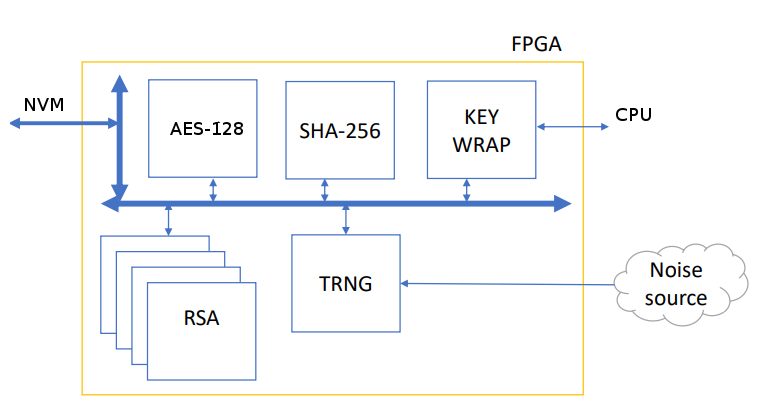
\includegraphics[width=0.8\linewidth]{pictures/hsm_architecture.png}
  \caption{Esquema general de un HSM para sistema embebido.}
  \label{fig:hsm_general}
\end{figure}

Los HSMs existen en diferentes configuraciones, los tipos de HSM comunes en sistemas embebidos se encuentran en forma de coprocesadores conectados mediante un bus de alto desempeño directamente al microcontrolador, igualmente se encuentran como un componente interno del microcontrolador. En las siguiente secciones se presenta la planeación del proyecto y la estratégia para realizar las pruebas y validación del mismo.

\begin{landscape}
\section{Planeación}

\noindent
\begin{ganttchart}[vgrid, hgrid, y unit title=0.8cm, y unit chart=0.8cm,
                   title label font=\footnotesize, bar label font=\small, 
                   bar label anchor/.append style={align=right}]{1}{36}
  \gantttitle{2020}{36}\\
  \gantttitle{Ene}{4}\gantttitle{Feb}{4}\gantttitle{Mar}{4}
  \gantttitle{Abr}{4}\gantttitle{May}{4}\gantttitle{Jun}{4}
  \gantttitle{Jul}{4}\gantttitle{Ago}{4}\gantttitle{Sep}{4}\\
  \gantttitle{s1}{1}\gantttitle{s2}{1}\gantttitle{s3}{1}\gantttitle{s4}{1}
  \gantttitle{s5}{1}\gantttitle{s6}{1}\gantttitle{s7}{1}\gantttitle{s8}{1}
  \gantttitle{s9}{1}\gantttitle{s10}{1}\gantttitle{s11}{1}\gantttitle{s12}{1}
  \gantttitle{s13}{1}\gantttitle{s14}{1}\gantttitle{s15}{1}\gantttitle{s16}{1}
  \gantttitle{s17}{1}\gantttitle{s18}{1}\gantttitle{s19}{1}\gantttitle{s20}{1}
  \gantttitle{s21}{1}\gantttitle{s22}{1}\gantttitle{s23}{1}\gantttitle{s24}{1}
  \gantttitle{s25}{1}\gantttitle{s26}{1}\gantttitle{s27}{1}\gantttitle{s28}{1}
  \gantttitle{s29}{1}\gantttitle{s30}{1}\gantttitle{s31}{1}\gantttitle{s32}{1}
  \gantttitle{s33}{1}\gantttitle{s34}{1}\gantttitle{s35}{1}\gantttitle{s36}{1}\\
  \ganttbar{Fundamento teórico}{1}{4}\\
  \ganttbar{Estado del arte}{4}{10}\\
  \ganttbar{Definición de ojetivos}{4}{5}\\
  \ganttbar{Propuesta de proyecto}{2}{5}\\
  \ganttbar{Ajuste de hipótesis}{11}{12}\\
  \ganttbar{Requerimientos}{12}{14}\\
  \ganttbar{Diseño del sistema}{14}{18}\\
  \ganttbar{Diseño de pruebas}{13}{15}\\
  \ganttbar{Desarrollo del sistema}{18}{22}\\
  \ganttbar{Pruebas unitarias}{22}{24}\\
  \ganttbar{Pruebas de integración}{24}{26}\\
  \ganttbar{Mejora del sistema}{26}{30}\\
  \ganttbar{Redacción de resultados}{30}{31}\\
  \ganttbar{Revisión y retroalimentación}{31}{36}
\end{ganttchart}
\end{landscape}

\section{Pruebas y validación}

\subsection{Introducción a UVM}

La funcionalidad de cada elemento de los \textit{testbenches} basados en UVM se explica en esta sección. Una prueba o \textit{test} UVM es la clase más alta dentro de la API. La prueba es responsable de configurar el banco de pruebas. El esquema general de una prueba en UVM se muestra en la Figura \ref{uvm_tb}, la abtracción mostrada en esta arquitectura permite la definición de pruebas a bajo o alto nivel sin cambios significativo.

\begin{figure}[h]
  \centering  
  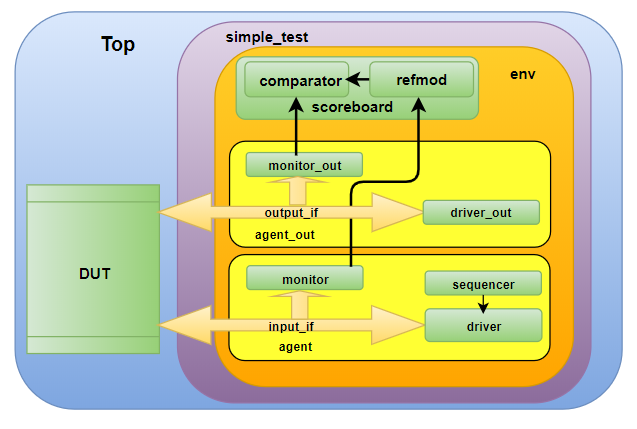
\includegraphics[width=0.8\linewidth]{pictures/uvm.png}
  \caption{Diagrama a bloques de un \textit{testbench} utilizando UVM.}
  \label{uvm_tb}
\end{figure}

\textbf{uvm agent:} Agrupa los componentes uvm específicos de una interfaz o protocolo.Por ejemplo, agrupa los componentes asociados con el BFM (\textit{Bus Functional Model}). Los componentes de un agente se definen en los siguientes párrafos.

\textbf{sequence item:} Define la actividad a nivel de pin generada por el agente, esto es, conducir al DUT (\textit{Design Under Test}) a través del controlador o la actividad monitoreada por el monitor.

\textbf{uvm driver:} Responsable de conducir los datos de nivel de paquete dentro del \textit{sequence item} al nivel de pin al DUT.

\textbf{uvm sequence:} Define la secuencia en la que los elementos de datos deben generarse y enviarse o recibirse desde y hacia el controlador.

\textbf {uvm sequencer:} Responsable de enrutar el paquete de datos (\textit{sequence item}) generado en secuencia hacia el controlador o viceversa.

\textbf{uvm monitor:} Observa la actividad de nivel de pin en las señales de la interfaz y se convierte en nivel de paquete que se envía a componentes como los \textit{scoreboards}.

\textbf{uvm scoreboard:} Recibe los elementos de datos del monitor y los compara con los valores esperados.
los valores esperados pueden ser valores de referencia (\textit{golden data}) o generados a partir del modelo de referencia.


\subsection{Herramienta de pruebas \textit{uvm-python-toolchain}}

Para este proyecto se encuentra en desarrollo una herramienta que permite la automatización de pruebas con UVM. La herramienta está escrita en Python y utiliza la librería unittest. Esta herramienta permite al desarrollador definir pruebas sobre un \textit{test model} escrito en UVM y simulado en Modelsim. Al final, uvm es el encargado de generar un reporte que es evaluado en la parte de Python y se determina el éxito o no de la prueba. En la Figura \ref{fig:run_test}, se muestra la secuencia principal de la herramienta en Python, este módulo ejecuta Modelsim con un argumento \textit{.do} que es la extensión del lenguaje \textit{scripting} de Modelsim.

\begin{figure}[h]
  \centering  
  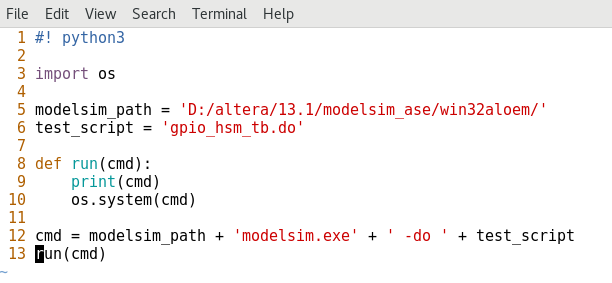
\includegraphics[width=0.8\linewidth]{pictures/python_test.png}
  \caption{Programa en Python que ejecuta todas las prruebas del \textit{test model}.}
  \label{fig:run_test}
\end{figure}

Esta herramienta será utilizada para la etapa de pruebas unitarias y de integración para facilitar el desarrollo, además, serán agregadas funcionalidades para análisis estático de código.

\newpage
\subsection{Pruebas unitarias}

\noindent \textbf{Definición}

La amplitud deseada en las pruebas unitarias será a nivel de algoritmo criptográfico. Es decir, se evaluará el \textit{hashing}, cifrado y generación de números aleatorios. Las técnicas a utilizar son caja blanca y la evaluación será, además, relacionada a cubrir los requerimientos técnicos del sistema. 

\noindent\textbf{Participantes}

\begin{itemize}
  \item El desarrollador
  \item El \textit{toolchain} que podrá correr pruebas automáticamente
\end{itemize}


\noindent\textbf{Metodología}

\begin{itemize}
  \item El componente que ejecuta un algoritmo criptográfico se separa en un \textit{testbench} UVM
  \item Se definen los estímulos para el algoritmo
  \item Se define la sequencia para transmitir los estímulos al DUT
  \item Se ejecuta la simulación UVM
  \item Se almacenan los resultados del scoreboard
  \item El programa que ejecuta las pruebas determina si la prueba tiene éxito o no
\end{itemize}


\subsection{Pruebas de integración}

\noindent\textbf{Definición}
Las pruebas de integración se enfocan a la prueba de algoritmos a alto nivel, es decir, se prueba un CMAC en lugar de probar directamenete el algoritmo de cifrado. Además, de manera incremental, se busca interconectar los componentes del HSM al controlador principal para que verificar que los resultados de la integración incremental tienen compatibilidad con niveles de integración a menor nivel de abstracción.

\noindent\textbf{Participantes}

\begin{itemize}
  \item El desarrollador
  \item El \textit{toolchain} que podrá correr pruebas automáticamente
\end{itemize}

\noindent\textbf{Metodología}


\begin{itemize}
  \item Los componentes que ejecutan un algoritmo de alto nivel como CMAC se separa (DUT) en un \textit{testbench} UVM
  \item Se definen los estímulos para el algoritmo, utilizando un modelo de referencia
  \item Se define la sequencia para transmitir los estímulos al DUT
  \item Se ejecuta la simulación UVM
  \item Se almacenan los resultados del scoreboard
  \item El programa que ejecuta las pruebas determina si la prueba tiene éxito o no comparando los resultados con el modelo de referencia
\end{itemize}

\subsection{Pruebas de sistema}

\noindent\textbf{Definición}
Las pruebas de sistema se enfocan a la prueba del sistema a nivel de servicios, es decir, se prueba una interrupción al controlador principal en lugar de probar directamenete el algoritmo CMAC.

\noindent\textbf{Participantes}

\begin{itemize}
  \item El desarrollador
  \item El \textit{toolchain} que podrá correr pruebas automáticamente
\end{itemize}

\noindent\textbf{Metodología}


\begin{itemize}
  \item El sistema completo se separa como DUT en un \textit{testbench} UVM
  \item Se definen los estímulos para el sistema como la interrupción y los argumentos del servicio criptográfico
  \item Se define la sequencia para transmitir los estímulos al DUT
  \item Se ejecuta la simulación UVM
  \item Se almacenan los resultados del scoreboard
  \item El programa que ejecuta las pruebas determina si la prueba tiene éxito o no comparando los resultados con el modelo de referencia y otros sistemas con la misma funcionalidad
\end{itemize}

\subsection{Análisis con herramientas \textit{Lint}}

\noindent\textbf{Verilator}

Verilator es una herramienta de análisis estático de código Verilog o SystemVerilog. Verilator se invoca con parámetros similares a \textit{gcc} o \textit{vlog} de Modelsim. El código Verilog o SystemVerilog sintetizable especificado como entrada es leído y se realizan comprobaciones de buenas prácticas, opcionalmente, se pueden insertar comprobaciones y puntos de análisis de cobertura.

\noindent El siguiente es un ejemplo de la ejecución de Verilator sobre linux:
%\begin{verbatim*}
\begin{lstlisting}
  $ verilator --lint-only -Wall file.v
\end{lstlisting}
%\end{verbatim*}
        
\newpage
\bibliographystyle{ieeetr}
\bibliography{bibliography}

\end{document}
